\documentclass[prl,onecolumn,amsmath,amssymb,superscriptaddress,notitlepage]{revtex4-1}
\usepackage{bm,psfrag,graphicx,setspace,color}
\usepackage{hyperref}
\hypersetup{
    colorlinks=true,
    linkcolor=black,
    filecolor=magenta,      
    urlcolor=blue,
    citecolor=black
}

%% Options and definitions
\linespread{1.0}
\selectfont
\definecolor{myred}{RGB}{145, 3, 3}
\definecolor{myblue}{RGB}{0, 84, 156}


\begin{document}
\title{Applicant evaluation --- Machine learning}
\date{\today}
\author{Niket Thakkar}
\email{thakkar@uw.edu}
\affiliation{Department of Applied Mathematics, University of Washington, Seattle, Washington 98195-3925, USA}
\maketitle

\section{Control Questions}

%%%%%% Question 1
{\color{myred}\textbf{Question 1:} Consider a hypothetical population composed of two subgroups: the easily accessible group, comprising $80\%$ of the population, and the difficult-to-access group, comprising the remaining $20\%$.  A series of three vaccination campaigns are targeted at this population --- in each campaign, only a single dose is given out to each recipient.  A member of the easily accessible group has a $90\%$ probability of receiving a dose in each campaign, and a member of the difficult-to-access group has a $40\%$ probability of receiving a dose. These probabilities of receiving a dose are independent in each campaign, but the accessibility group membership is stable (i.e., if a person is in the easily accessible group, they remain in that group through all $3$ campaigns). Please fill out the following table describing the dose distribution (the fraction of the TOTAL population that has received $1$, $2$, $3$ doses) after each campaign.}
\\

\begin{figure}[h!]
\centering
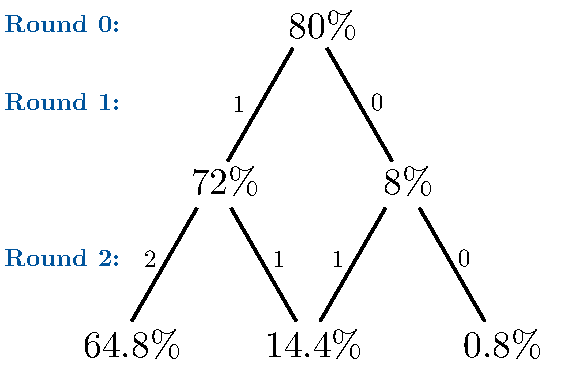
\includegraphics[scale=0.75]{q1_v2.pdf}
\caption{Decision tree to visualize vaccination campaigns on the easily accessible population. Each split increases the number of doses by 1 or leaves it the same with probability $p=0.9$ and $1-p=0.1$ respectively. This type of tree is a common visualization of a series of Bernoulli trials and indicates how the solution can be written for general $p$.}\label{tree}
\end{figure}
An approach to this problem is described visually in Fig. \ref{tree}. Here, I show the effect of the first two vaccination campaigns on the easily accessible population ($80\%$ of the total population). Each round the populations independently split into two, one which gets a vaccine dose and another which does not. Since the probability of receiving a dose for this population is $0.9$, the majority of this population receive two doses after two campaigns. 

Fig. \ref{tree} is a common visualization of a series of Bernoulli trials \cite{downey2014}, where the probability of exactly $k$ successes (doses) in $n$ independent experiments (campaigns) with success probability $p$ is

\begin{equation}
\begin{split}
P(k|n,p) &= \begin{pmatrix} n \\ k \end{pmatrix}p^k(1-p)^{n-k} \\
&= \frac{n!}{k!(n-k)!}p^k(1-p)^{n-k}, \label{fixed_p}
\end{split}
\end{equation}
\\
where the binomial coefficient prefactor accounts for multiple paths to the same number of successes, as shown in Fig. \ref{tree} for the single dose ($k=1$) case. This formula can be applied to the easily accessible and difficult-to-access populations independently since we assume group membership is stable. The solution is presented in Table \ref{table}.
\begin{center}
\begin{table}[h!]
\def\arraystretch{1.5}
\setlength\tabcolsep{0.25in}
\begin{tabular}{| c | c | c | c | c |}
\hline
 & 0 doses & 1 dose & 2 doses & 3 doses \\
\hline
Before Round 1 & 100$\%$ & 0$\%$ & 0$\%$ & 0$\%$ \\
\hline
After Round 1 & 20$\%$ & 80$\%$ & 0$\%$ & 0$\%$ \\
\hline
After Round 2 & 8$\%$ & 24$\%$ & 68$\%$ & 0$\%$ \\
\hline
After Round 3 & 4.4$\%$ & 10.8$\%$ & 25.2$\%$ & 59.6$\%$ \\
\hline
\end{tabular}
\caption{Table of the percentage of the total population with $k=0$, 1, 2, and 3 vaccine doses after each campaign. These are computed by calculating the success probability in each population ($80\%$ with $p=0.9$ and $20\%$ with $p=0.4$) and taking the population percentage weighted sum of the results.}\label{table}
\end{table}
\end{center}

%%%%%% Question 2
{\color{myred}\textbf{Question 2:} Now instead of only two groups, consider a population in which each individual has their own probability $p$ of receiving a dose in a given round.  The distribution of these probabilities across the population is some probability distribution function $f(p)$ for  $p\in[0, 1]$. Please write an equation describing the marginal distribution of doses in the population after $n$ campaigns --- that is, the probability $P(k| n)$ that a random individual drawn from this population has received $k$ doses after $n$ campaigns, marginalizing over $p$.}
\\

It is helpful to consider the special case where $p$ is deterministic, and $f(p)=\delta(p-p')$, where $\delta$ is the Dirac delta function and $p'$ is the constant probability of an individual receiving a dose. This simplified situation is what we considered for each population in the first question -- in one case, $p'=0.9$ and in the other $p'=0.4$. This indicates that Eq. \ref{fixed_p} is a good starting point.

$f(p)$ is then, more generally, the weight associated with each value of $p\in[0,1]$. Thus, the probability can be written as the $f(p)$ weighted average of Bernoulli trials for each $p$,

\begin{equation}
P(k|n,f(p)) = \int_0^1 dp f(p)\left(\frac{n!}{k!(n-k)!}p^k(1-p)^{n-k} \right).
\end{equation}
\\
As it should, when $f(p)=\delta(p-p')$, this distribution reduces to Eq. \ref{fixed_p}. For more general $f(p)$ this distribution can instead be calculated by standard numerical methods. 
\\

%%%%%% Question 3
{\color{myred}\textbf{Question 3:} Certain vaccines (e.g., DTP) are given to infants at $6$, $10$, and $14$ weeks in some countries, and scheduled for $2$, $4$, and $6$ months in others.  In a couple of paragraphs, please describe some reasons why different immunization timings may be appropriate in different contexts.}
\\

Determining the optimal immunization schedule in different contexts is a difficult problem and is a subject of current research \cite{gentile2010,cunliffe2016}. Region-to-region, immunization timings must be determined to weigh disease burden with vaccine safety, effectiveness, side-effects, and cost. 

In a country with good infrastructure and high vaccine coverage, timings can be more spread out, allowing the vaccine to safely take effect in a patient and lowering the burden on patients. This is especially true in areas where disease prevalence is low compared to coverage, since the so-called herd effect can protect people who have yet to receive the vaccine. On the other hand, in countries where vaccine coverage is low relative to disease prevalence, and people are more difficult to reach, either because of poor infrastructure or high cost, immunization timing can be accelerated to promote a herd effect quickly. This acceleration, however, needs to be weighed against side effects and effectiveness of the vaccine itself, which usually needs some incubation period in a patient.
\\


\section{Challenge Question --- vaccination coverage from survey data}

In this section, I model polio vaccination coverage using logistic regression on the provided Nigerian family survey data (\verb|data.csv|), which asks families a number of general questions about a child's household, family members, and health. Code used to generate the figures and tables can be found in the attached Python files, \verb|load_data.py|, \verb|basic_data_analysis.py|, \verb|statsmodels_logit.py|, and \verb|theano_logit.py|. Running the code requires a handful of Python libraries (most importantly \verb|numpy|, \verb|scipy|, \verb|matplotlib|, \verb|pandas| \cite{mckinney2011}, \verb|statsmodels| \cite{seabold2010}, and \verb|theano| \cite{theano2016}), all of which can be found in the \href{https://www.continuum.io/downloads}{Anaconda Python distribution}. 

\subsection{Basic Data Analysis}

\begin{figure}[h!]
\centering
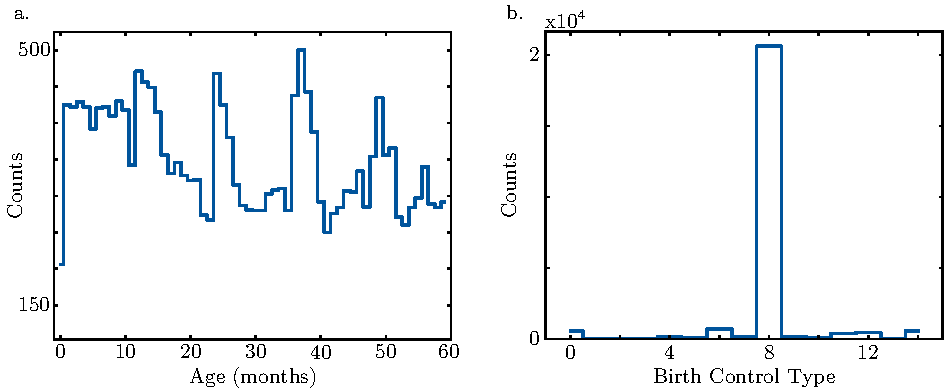
\includegraphics[scale=0.9]{age_histogram.pdf}
\caption{(a) Histogram of child's age in months, showing roughly evenly distributed ages. (b) Histogram of birth control methods of the respondent with different methods assigned numbers (see code for details). This shows that birth control is not very informative since it is concentrated in one type, explaining why logistic regression of birth control method to predict vaccine coverage is ill-conditioned.}\label{histograms}
\end{figure}

\verb|load_data.py| contains functions to import the data and header information as a \verb|pandas| DataFrame and a hash table. The dataset has a total of $23900$ entries, each corresponding to a different child. Using the headers, I can see that column \verb|b5| is a yes or no question asking if the child was alive at the time of the survey, and slicing the dataset for yes answers shows that $21673$ were alive, about $90.7\%$ of the total. The dataset has $73$ columns, each corresponding to a question, identifier, or statistical weight associated with that child. For instance, using column \verb|hw1|, I can create the histogram of the children's ages (in months) shown in Fig. \ref{histograms}a. This plot shows that the ages are roughly evenly distributed between $0$ and $5$ years-old, with slightly more representation at younger ages. 

The histogram in Fig. \ref{histograms}a discards not-a-number (\verb|NaN|) values, amounting to $2978$ entries, $75\%$ of which are associated with children who are not alive at the survey time. Since the dataset is large, I can construct a valid model of vaccination coverage without \verb|NaN| data, and I continue to neglect \verb|NaN| values throughout the modeling and analysis below.

Fig. \ref{histograms}a also neglects the unequal sample weighting given in column \verb|v005|. This weighting is likely due to deliberate oversampling of certain demographics in Nigeria in order to improve the statistical power of tests performed on the dataset, and the number in this column corresponds to the number of people in the Nigerian population represented by that entry \cite{downey2014}. Neglecting these weights effectively treats that data as a representative sample of the total population, which is purposefully not the case. 

Although the unequal sample weights can be handled by weighted resampling of the dataset, I will neglect sample weights to simplify the analysis. I have, however, build a resample option into the \verb|LoadData()| function, and this can be used to verify that the sample weights do not significantly effect the logistic regression and results discussed below. 


\subsection{Data Preprocessing and Choosing a Method}

To model polio vaccine coverage for Nigerian children, I need to create a classification model which takes some subset of the data and predicts the value of columns \verb|h0| and \verb|h8|, categorical data which indicate whether a child has had a first dose of polio vaccine and a full schedule of polio vaccine respectively. 

In the raw data, \verb|h0| and \verb|h8| can take values of either $0, 1, 2, 3, 8,$ and $9$. As described in the header information, $0$ means no, $1$ means yes, and $2$ and $3$ mean yes but with uncertainty in the date or validity of the answer. Meanwhile, $8$ means the respondent did not know and $9$ is a missing entry. Before modeling vaccine coverage, I make one more simplifying assumption: I treat $1$, $2$, and $3$ all as $1$, and I convert $8$ and $9$ to \verb|NaN|. This transformation is applied to the polio and measles vaccine (\verb|h9|) columns and simplifies the problem by turning it into a binary classification. In the conclusion, I discuss a method to handle multiple classification categories and avoid this simplifying assumption.

There are numerous methods to handle binary classification problems like this. Two options are:
\begin{enumerate}
\item \textbf{Random Forests:} Random forests are a set of parameterized decision trees \cite{breiman2001,kuhn2013} which work especially well on categorical predictors, as is the case for most of the dataset here. They have a strong track record of success, and they are robust to nonlinear relationships between predictors. They can, however, be difficult to gain insight from, and models, although accurate, can become quite complicated.

\item \textbf{Logistic Regression:} Logistic regression is a linear classification method which is based on regression of the odds of data belonging to a certain class \cite{downey2014,hastie2011}. Although it is a linear regression, the logistic model performs remarkably well in many cases while remaining simple enough to interpret. If accuracy with logistic regression is a problem, logistic models can be used as neurons in a deep network to capture more complicated phenomena and nonlinearity, much like decision trees are grouped into random forests. 
\end{enumerate}

As mentioned above, I chose logistic regression for this problem. Starting with the simplest model that can perform well is an important first step in analyzing a dataset, and as I will demonstrate below, the parameterized logistic model can be used to tell us which states in Nigeria are more or less likely to have vaccination coverage. This important and interesting insight would be difficult to get from more complicated classification methods.

\subsection{Strongest Predictors}

To choose the best $5$ predictors from the $\sim 70$ options in the dataset, I computed single predictor logistic regressions for each predictor and calculated the pseudo $R^2$ value \cite{mcfadden1973}, which is a measure of the predictive power of the model and relative likelihood of each model. This is certainly not the only approach -- one could for instance use a singular value decomposition to get the best linear combinations of predictors \cite{kuhn2013} -- but this is a simple and effective method which retains our ability to interpret the fitted model.

This test is performed using the \verb|statsmodels| library in the function \verb|PredictivePower()|. Output from this function when \verb|h0| is the dependent variable looks something like this:
\begin{verbatim}
[R^2, column name, p-value, description]
[0.18465364789771355, 'h9', 0.0, 'Has received measles vaccine']
[0.18400464124597882, 'sstate', 0.0, 'State of residence']
[0.16890706453096416, 'v106', 0.0, 'Highest education level']
[0.16498917268367252, 'v133', 0.0, 'Total years of education']
[0.16461757378735575, 'v190', 0.0, 'Wealth index']
[0.13016838796474628, 'v024', 0.0, 'Region']
[0.11326662473826232, 'v155', 0.0, 'Literacy code']
[0.09979484208624656, 'latnum', 0.0, 'Latitude of household (noise added to protect identities)']
[0.086802812765456316, 'v511', 0.0, 'Age at first cohabitation']
[0.071037836233419083, 'v025', 0.0, 'Urban/Rural']
\end{verbatim}
ranking each predictor by $R^2$. The results are somewhat intuitive, indicating that having had a first dose polio vaccination can be determined by whether a child has had a measles vaccine, where they live, or the education history of their parents. When the same test is run with \verb|h8| as the dependent variable, I get similar results,
\begin{verbatim}
[R^2, column name, p-value, description]
[0.071552567043899562, 'sstate', 0.0, 'State of residence']
[0.067779468044237401, 'h9', 0.0, 'Has received measles vaccine']
[0.023488264031127914, 'v024', 9.4119174658534212e-147, 'Region']
[0.014596011654842922, 'hw1', 4.6988803740341658e-92, "Child's age in months"]
[0.013996075518395767, 'b2', 2.4272438874562254e-91, 'Year of birth']
[0.013339881258623065, 'longnum', 3.7842161859623254e-87, 'Longitude of household (noise...)']
[0.01249991945062856, 'slang2', 8.8271212213074903e-82, "respondent's native language code"]
[0.0075284874093249909, 'var1', 5.5250402117415408e-50, 'var1']
[0.0070508340247524837, 'v106', 1.3212272918699565e-44, 'Highest education level']
[0.0066753287461716049, 'v190', 2.8049612481902739e-41, 'Wealth index']
\end{verbatim}
but with significantly lower $R^2$ across the board, indicating that the coverage of the full-schedule of polio vaccine is more difficult to predict. 

Interestingly, not all of the single predictor logistic regressions converge. For example, \verb|v312|, which asks the respondent's birth control method, cannot be used to predict polio vaccine coverage with a logistic model and this dataset. To understand why, I made the histogram of \verb|v312| shown in Fig. \ref{histograms}b. Since the data is so strongly concentrated on a single method, \verb|v312| is simply not informative enough to parameterize the regression. This is also the case for the other predictors where the test fails to converge. For our purposes, we can simply ignore these parts of the data.

Many of the predictors in the top $10$ for each dependent variable are correlated, as can be shown using the \verb|CorrelationMatrix()| function I have provided. For instance, state-of-residence (\verb|sstate|) and region (\verb|v024|) likely give redundant information. Taking this into account, I chose my top predictors to be \verb|h9| (whether the child has measles vaccine), \verb|sstate| (the child's home state), \verb|v106| (respondent's education level), \verb|v190| (respondent's wealth index), and \verb|hw1| (child's age).
 

\subsection{Logistic Regression Performance and Discussion}

\begin{figure}[h!]
\centering
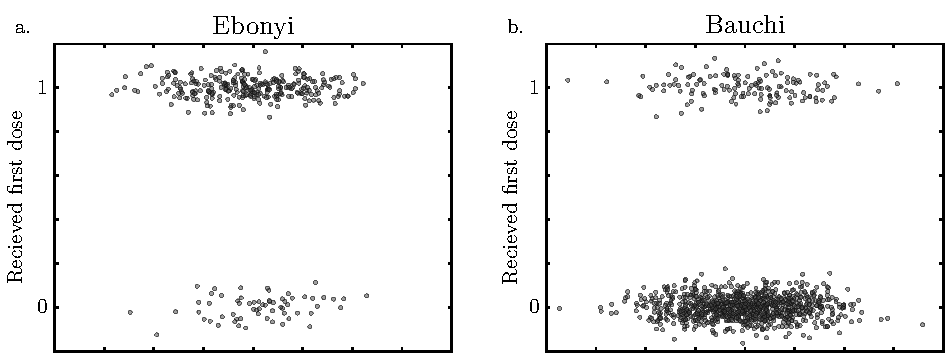
\includegraphics[scale=0.9]{scatter_plots.pdf}
\caption{(a) Scatter plot of first vaccine dose in two different states with added noise for clarity. (a) In Ebonyi, the group that has received a first dose of polio vaccine is much larger than the group that has not, in qualitative agreement with the coefficient found in the logistic regression. (b) The opposite is true in Bauchi, indicating the Bauchi maybe a state which needs more attention.}\label{scatterplots}
\end{figure}

\verb|statsmodels_logit.py| provides my logistic regression class to do the full $5$ predictor regression on the dataset. The script provides functions to save its state and be reused on other datasets of the same form. 

Before parameterization, the data is randomized and split into a training set ($60\%$) and a test set ($40\%$). Parameterization of the model yields a summary which, for the \verb|h0| regression, includes a table like this:
\begin{verbatim}                 
=========================================================================================
                            coef    std err          z      P>|z|      [95.0% Conf. Int.]
-----------------------------------------------------------------------------------------
Intercept                 0.9031      0.219      4.132      0.000         0.475     1.331
sstate[T.ADAMAWA]        -0.1188      0.214     -0.556      0.579        -0.538     0.300
sstate[T.AKWA IBOM]      -0.6907      0.229     -3.010      0.003        -1.140    -0.241
sstate[T.ANAMBRA]        -0.2957      0.240     -1.234      0.217        -0.765     0.174
sstate[T.BAUCHI]         -1.6357      0.224     -7.313      0.000        -2.074    -1.197
sstate[T.BAYELSA]        -1.6470      0.224     -7.364      0.000        -2.085    -1.209
sstate[T.BENUE]          -0.2465      0.235     -1.049      0.294        -0.707     0.214
sstate[T.BORNO]          -1.0183      0.251     -4.058      0.000        -1.510    -0.526
sstate[T.CROSS RIVER]    -0.6000      0.245     -2.445      0.014        -1.081    -0.119
sstate[T.DELTA]          -1.3827      0.223     -6.204      0.000        -1.820    -0.946
sstate[T.EBONYI]          1.2884      0.254      5.068      0.000         0.790     1.787
...
v106[T.No education]     -1.1667      0.122     -9.526      0.000        -1.407    -0.927
v106[T.Primary]          -0.8153      0.119     -6.828      0.000        -1.049    -0.581
v106[T.Secondary]        -0.3689      0.113     -3.263      0.001        -0.590    -0.147
v190[T.Poorer]           -0.3425      0.062     -5.496      0.000        -0.465    -0.220
v190[T.Poorest]          -0.6831      0.073     -9.403      0.000        -0.825    -0.541
v190[T.Richer]            0.3769      0.064      5.919      0.000         0.252     0.502
v190[T.Richest]           0.9260      0.082     11.301      0.000         0.765     1.087
hw1                      -0.0227      0.001    -17.702      0.000        -0.025    -0.020
h9                        2.0666      0.049     41.809      0.000         1.970     2.164
=========================================================================================
\end{verbatim}

As mentioned earlier, these coefficients lend insight into the vaccine coverage in Nigeria. For example, we see that having had a measles vaccine is a strong indicator that a child has a polio vaccine since the coefficient is large and positive and has low uncertainty. More than that, we see a breakdown of Nigeria by state showing where to find lower and higher probability of having had the first polio vaccine. For instance, families in Ebonyi are much more likely to have vaccine coverage than those in Bauchi. This is depicted in Fig. \ref{scatterplots}a and b, where scatter plots with added noise produce groups of data with and without coverage in each state. Families in Ebonyi with vaccine coverage vastly outnumber those without, while the opposite is true in Bauchi. In this way, this simple logistic regression model can be used to identify areas where coverage is needed. 

Methods for error testing are also provided in \verb|statsmodels_logit.py|. With the parameterization above, the model has $\sim 80.2\%$ accuracy for predicting \verb|h0| in the test set. If the logistic regression with the same predictors is reparameterized and tested on the \verb|h8| data, the accuracy falls to $\sim 70.0\%$. This fall should be expected based on the pseudo $R^2$ tests above, which indicated that the full polio vaccine schedule data was more difficult to predict.

\subsection{Conclusion}

I have presented a logistic regression model which takes five inputs and predicts whether a Nigerian child has had a first course or full-schedule of polio vaccine. The model's performance is likely not good enough to move forward, and additional complexity is needed to increase the accuracy on test data. One serious drawback of the model is that it is linear, and I have no reason to expect a linear relationship between the predictors and vaccine coverage. 

As mentioned above, it is possible to link logistic regressions in a deep network. This is a good option for increasing accuracy but suffers from increased computational complexity. Towards this end, I have included an adaptation of \href{http://deeplearning.net/tutorial/logreg.html}{Theano's logistic regression} for the MNIST handwriting data suitable for the dataset considered here. This second implementation not only serves as a check on the results above but is written to handle multiple classifications in the dependent variable (avoiding the simplifying assumption above) and can be run on a GPU, significantly increasing performance. This increase in performance is critical if one wants to network these regression classes into a more complex model. 

\begin{thebibliography}{1}
\bibitem{downey2014} Downey, Allen B. \emph{Think stats}. O'Reilly Media, Inc., 2014.
\bibitem{gentile2010}Gentile, Angela, et al. \emph{Pediatric disease burden and vaccination recommendations: understanding local differences}. International Journal of Infectious Diseases 14.8 (2010): e649-e658.
\bibitem{cunliffe2016}Cunliffe, Nigel A., and Gagandeep Kang. \emph{Can Changes to Scheduling Enhance the Performance of Rotavirus Vaccines in Low-Income Countries?}. Journal of Infectious Diseases 213.11 (2016): 1673-1675.
\bibitem{mckinney2011}McKinney, Wes. \emph{pandas: a foundational Python library for data analysis and statistics}. Python for High Performance and Scientific Computing (2011): 1-9.
\bibitem{seabold2010}Seabold, Skipper, and Josef Perktold. \emph{Statsmodels: Econometric and statistical modeling with python.} Proceedings of the 9th Python in Science Conference. 2010.
\bibitem{theano2016} The Theano Development Team, et al. \emph{Theano: A Python framework for fast computation of mathematical expressions.} arXiv preprint arXiv:1605.02688 (2016).
\bibitem{breiman2001} Breiman, Leo. \emph{Random forests}. Machine learning 45.1 (2001): 5-32.
\bibitem{kuhn2013} Kuhn, Max, and Kjell Johnson. \emph{Applied predictive modeling}. New York: Springer, 2013.
\bibitem{hastie2011}Trevor J.. Hastie, Robert John Tibshirani, and Jerome H. Friedman. \emph{The elements of statistical learning: data mining, inference, and prediction}. Springer, 2011.
\bibitem{mcfadden1973} McFadden, Daniel. \emph{Conditional logit analysis of qualitative choice behavior}. (1973): 105.






\end{thebibliography}


\end{document}